	
%\part{Projetos menores}
%	\chapter{Estudo sobre regiões Maxwellianas nos perfis de viscosidade}
%	\chapter{Comparação de ITC de MG em dois sentidos opostos}
	
\part{Contribuições para outros projetos}

	\chapter{Breve descrição sobre o projeto de fibrose cística}

	Durante a execução do projeto de doutorado, foi estabelecida uma parceria com uma aluna de doutorado da Faculdade de Ciências Médicas na Unicamp, Carla Cristina S. Gomez, através do Professor Francisco Benedito Pessine, do Instituto de Química da Unicamp, para a análise de amostras de muco de pacientes com fibrose cística. Foram realizadas medidas de curva de fluxo e da reologia oscilatória de amostras de muco de pacientes com a doença genética chamada fibrose cística. Essa doença afeta X\% da população, sendo mais prevalente entre os grupos A e B (X\%) do que outros.
	
	Essa doença possui vários níveis de gravidade, e afeta bastante negativamente o desenvolvimento corporal. Geralmente, os pacientes possuem pequena estatura e baixo peso, pela dificuldade do corpo de absorver alimentos, e pelos problemas respiratórios. Bastante escarro é produzido pelos pulmões, que não é liberado corretamente, sendo então expelido como escarro, após tosse, o que também acaba ferindo o pulmão. Infecções bacterianas são frequentes nos pacientes de fibrose cística. Os casos mais graves necessitam de transplante pulmonar para conseguir sobreviver.
	
	Trabalhos anteriores observaram que na fibrose cística, há um problema nas enzimas/proteínas XYZ, que controlam os processos de transporte de ABC. Logo, imaginou-se que a reinserção do íon bicarbonato poderia aliviar os sintomas respiratórios. Isso foi realizado com a inalação de amostras de bicarbonato de sódio. Foram coletadas amostras antes da inalação, e após a inalação de bicarbonato, a cada 30 minutos. Cada paciente retornava para casa, continuava a inalação, e retornava para acompanhamento, e mais coleta de muco, a cada semana. As amostras de muco eram coletadas em tubos Falcon, o pH era medido, e depois eram mantidas refrigeradas, de modo a impedir a proliferação de bactérias. Entre 24-48h após a coleta, as amostras eram analisadas no reômetro.

	\chapter{Contribuições ao projeto}
	
	Nesse projeto, foram analisados tanto curvas de fluxo, como a reologia oscilatória do muco. Utilizou-se tanto o reômetro Haake RheoStress1 quanto o Haake Mars III, ambos da Thermo Scientific, para as análises. Para o tratamento de dados, foi utilizado a linguagem Python, que permite resultados consistentes e de melhor qualidade, se comparados com o ajuste manual.
	
		\section{Determinação dos parâmetros de análise}
		
		Foram analisadas algumas amostras inicialmente para se determinar a faixa necessária ... % todo: terminar
	
		\section{Criação de um software para tratamento de curvas de fluxo}
		\label{sec:apn_tratamento_CF}
		Para o tratamento de dados de curva de fluxo, foi criado um programa que permite o usuário aplicar três modelos mais complexos e um modelo simplificado para a obtenção de valores de viscosidade no repouso. Todas as amostras de muco, sem exceção, demonstraram ser pseudoplásticas, então não foram colocados mais modelos. A seguir, será mostrado os modelos utilizados e seções da lógica do programa, pois o código fonte inteiro é longo demais para ser incluido aqui (aproximadamente 1000 linhas).
		
			\subsection{Modelos de curvas de fluxo pseudoplásticas}
			
		\label{sec:modelagem_curva_fluxo}
		Foram implementados os modelos de \emph{Carreau-Yasuda} (Eq \ref{eqn:AP_CarreauYasuda}), \emph{Carreau} (Eq. \ref{eqn:AP_Carreau}), \emph{Cross} (Eq. \ref{eqn:AP_Cross}) e \emph{linear}, de maior para menor complexidade, respectivamente. Os modelos correlacionam a taxa de cisalhamento (\(\dot{\gamma}\), variável independente) à viscosidade (\(\eta\), variável dependente) utilizando alguns parâmetros.
		
		\begin{equation}
		\eta = \eta_{\infty} + \frac{\eta_0 - \eta_{\infty}}{\left[  1 + \left(  \dfrac{\dot{\gamma}}{\dot{\gamma}_b}  \right)^{a}  \right]^{\frac{ \left(  n - 1  \right) }{a}}}
		\label{eqn:AP_CarreauYasuda}
		\end{equation}
		
		\begin{equation}
		\eta = \eta_{\infty} + \frac{\eta_0 - \eta_{\infty}}{\left[  1 + \left(  \dfrac{\dot{\gamma}}{\dot{\gamma}_b}  \right)^{2}  \right]^{\frac{n}{2}}}
		\label{eqn:AP_Carreau}
		\end{equation}
		
		\begin{equation}
		\eta = \eta_{\infty} + \frac{\eta_0 - \eta_{\infty}}{1 + \left(  \dfrac{\dot{\gamma}}{\dot{\gamma}_b}  \right)^{n}}
		\label{eqn:AP_Cross}
		\end{equation}
		
		O modelo linear considera somente valores de viscosidade em \(\dot{\gamma}\) próximos de zero, ou seja, \(\eta = \eta_0 + 0 \times \dot{\gamma}\).
		
		Os parâmetros possuem os seguintes significados:
		
		\begin{table}[H]
			\IBGEtab{%
				\caption{Parâmetros dos modelos de fluidos pseudoplásticos}
				\label{tab:params_pseudoplasticos}
			}%
			{%
				\begin{tabular}{c c p{9cm}}
					\toprule
					    Parâmetro      & Unidade   & Significado                                                       \\ \midrule
					    \(\eta_0\)     & Pa.s      & Viscosidade no repouso*                                           \\
					\(\eta_{\infty}\)  & Pa.s      & Viscosidade no infinito                                           \\
					      \(n\)        & --        & Inclinação da região de decaimento de viscosidade                 \\
					\(\dot{\gamma}_b\) & s\menosUm & \(\dot{\gamma}\) de início da região de decaimento de viscosidade \\ \midrule
					      \(a\)        & --        & Afeta tanto a inclinação quanto o ponto de inflexão               \\ \bottomrule
				\end{tabular}%
			}{}
		\end{table}
		% todo: pensar em colocar os gráficos mostrando como esses parâmetros afetam as curvas
		% todo: pensar um pouco mais sobre o Carreau-Yasuda e como que o a deve se comportar
		
		A Fig. \ref{fig:reologia_modelos} exemplifica os modelos de Carreau e Cross e como os parâmetros afetam o formato das curvas. Note que a escala dos eixos é logarítmica. Vemos que, essencialmente, ambas as curvas possuem formatos muito semelhantes, com os parâmetros escolhidos. A escolha de um modelo depende da qualidade dos dados e do desejo do experimentalista. Observando-se como os modelos variam com os parâmetros, nota-se que a queda de viscosidade do modelo de Carreau é menos abrupta que no modelo de Cross e se assemelha mais aos dados estudados, então esse modelo foi mais utilizado.
		
		\begin{figure}[H]
			\begin{subfigure}[t]{0.45\textwidth}
				\centering
				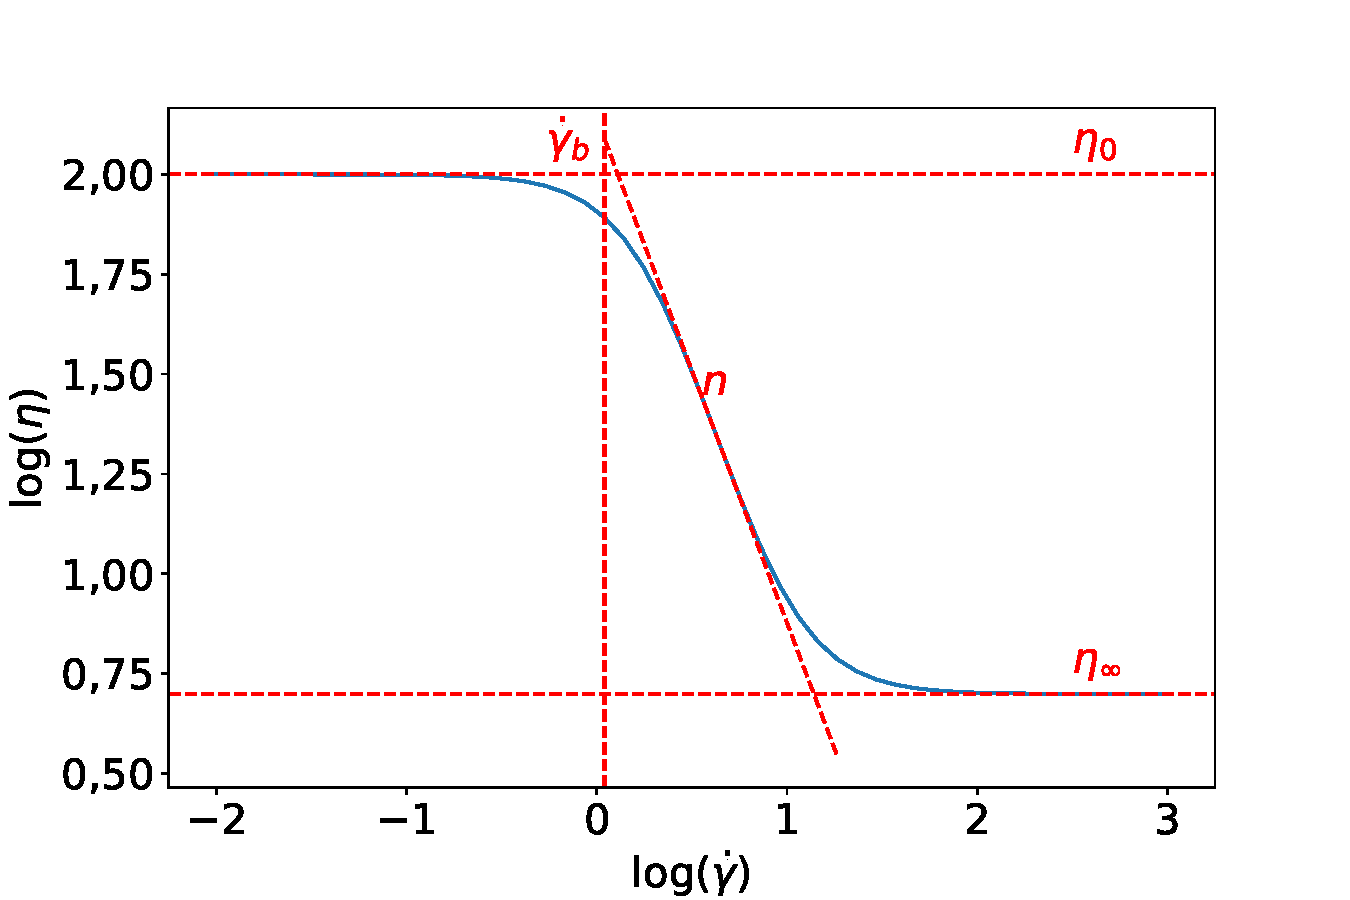
\includegraphics[width=\textwidth]{./imagens/reologia/Carreau}
				\caption{Modelo de Carreau}
				\label{fig:reologia_modelo_carreau}
			\end{subfigure} \qquad %
			\begin{subfigure}[t]{0.45\textwidth}
				\centering
				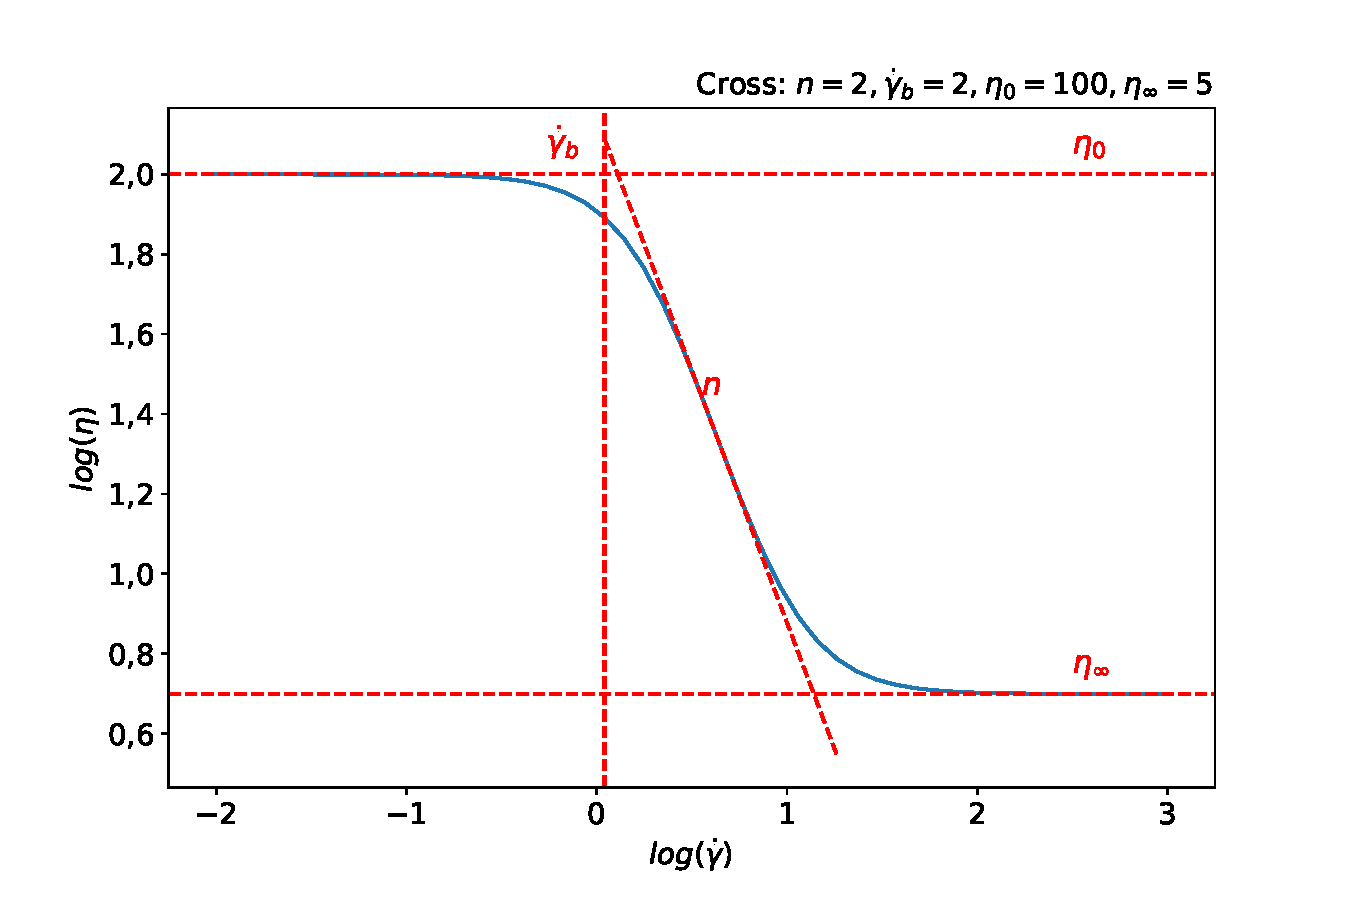
\includegraphics[width=\textwidth]{./imagens/reologia/Cross}
				\caption{Modelo de Cross}
				\label{fig:reologia_modelo_cross}
			\end{subfigure}
			\caption{Exemplos de curvas de fluxo descritas pelos modelos de Carreau e Cross, com os parâmetros utilizados.}
			\label{fig:reologia_modelos}
		\end{figure}
		
		De maior interesse para os estudos neste trabalho é a viscosidade no repouso, \(\eta_0\), e portanto esse é o foco do programa. Porém, o ajuste indiscriminado de um modelo a um dado experimental é problemático caso a qualidade do dado não seja boa, seja pela própria característica da amostra, ou pela sensibilidade do equipamento. Por exemplo, é frequente que apareçam artefatos de medida em baixos valores de \(\dot{\gamma}\), resultando ou num decréscimo ou acréscimo gradual de \(\eta\). Além disso, é possível que não seja observada a região descrita por \(\eta_{\infty}\), em altos valores de \(\dot{\gamma}\), o que atribui grande incerteza na determinação desse parâmetro. Dessa forma, é necessário que uma região das curvas seja escolhida para que o ajuste seja bem sucedido e informativo, o que representa a maior dificuldade nesse tipo de análise, devido à certa subjetividade no critério de escolha da região de ajuste.
		
		Por essa razão, e outras, como velocidade de análise, foi escrito o método de ajuste. O método consiste em realizar ajustes sucessivos, entre um ponto inicial \(P_i\) até um ponto final \(P_f\), e depois comparar os resultados dos ajustes para escolher um deles. Podem ser comparados, por exemplo, os parâmetros \(R^2\), \(\chi^2\) ou \(\chi_{red}^2\). Escolhido o melhor ajuste, observando-se, por exemplo, a maior proximidade de \(R^2\) a 1 ou de \(\chi^2\) a 0, tomando cuidado para não escolher uma faixa muito estreita de pontos, os resultados são graficados, gravados num arquivo de texto e passa-se para o próximo dado experimental.
		
		A listagem \ref{lst:exemplo_curva_de_fluxo} mostra duas seções do código completo do programa, uma mostrando o ciclo de ajuste utilizando o ajuste linear e \texttt{curve\_fit} e outro que realiza um ajuste não-linear utilizando o modelo de Carreau e \emph{lmfit}.
		
		\begin{listing}[H]
			\inputminted{python}{./python/curva_de_fluxo.py}
			\caption{Seções do código mostrando o método de ajuste}  % todo: encontrar um nome melhor
			\label{lst:exemplo_curva_de_fluxo}
		\end{listing}
		
		Essas funções estão dentro de uma classe chamada \texttt{Fitter}. Para utilizar essa classe em outros códigos, é necessário inicializar uma instância da classe \texttt{Settings} e depois inicializar uma instância da classe \texttt{Fitter} utilizando as configurações da classe \texttt{Settings}. Caso não haja um arquivo \texttt{settings.dat} na pasta, um arquivo com valores padrão será criado. Após isso, é possível tanto editar o arquivo \texttt{settings.dat} quando utilizar as funções \texttt{print\_settings, edit\_settings} do objeto \texttt{Settings}. Ao criar um objeto \emph{Fitter}, por padrão os ajustes configurados já são realizados e os resultados são mostrados na tela. Caso se deseja criar um gráfico mostrando o resultado dos ajustes, pode-se chamar a função \texttt{plot\_error\_graphs()}. 
		
		A listagem \ref{lst:exemplo_fitter} mostra como o programa pode ser utilizado por outros scripts, e o resultado do ajuste se encontra na Fig. \ref{fig:reologia_dado-exemplo}
		
		\begin{listing}[H]
			\inputminted{python}{./python/uso_fitter.py}
			\caption{Exemplo de como utilizar a ferramenta de ajuste não linear}  % todo: encontrar um nome melhor
			\label{lst:exemplo_fitter}
		\end{listing}
		
		\begin{figure}[H]
			\centering
			\includegraphics[width=\textwidth]{imagens/reologia/Dado-exemplo}
			\caption{Figura resultante do ajuste não linear de Carreau e ajuste linear gerada pela função \texttt{plot\_error\_graphs()}. As barras de erro são oriundas da propagação de erro dos parâmetros e os números em vermelho indicam os pontos iniciais e finais considerados em cada ajuste.}
			\label{fig:reologia_dado-exemplo}
		\end{figure}
		
		Note que no dado utilizado, não há muitos problemas de desvio da curva, então os ajustes foram bem comportados. Os exemplos das figuras \ref{fig:reologia_dado-problemadescida} e \ref{fig:reologia_dado-problemasubida} mostram problemas reais na região de baixos valores de \(\dot{\gamma}\).
		
		\begin{figure}
			\centering
			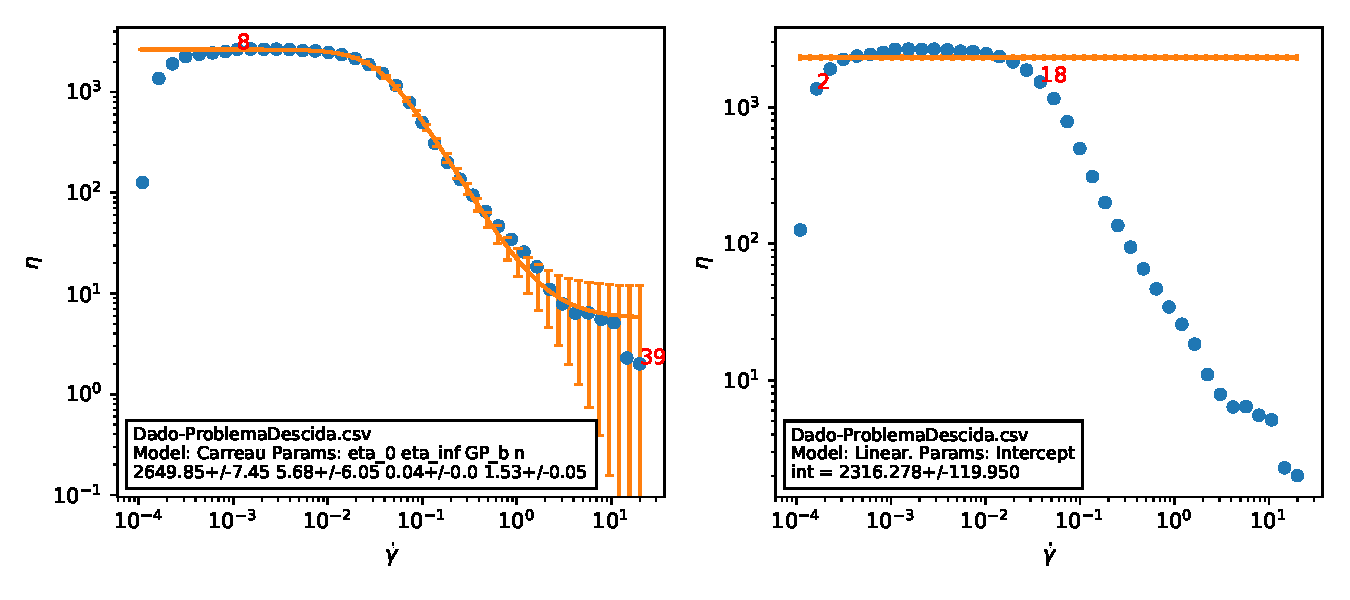
\includegraphics[width=\textwidth]{imagens/reologia/Dado-ProblemaDescida}
			\caption{Exemplo dos ajustes não-linear e linear de um dado real que possui uma queda nos valores de \(\eta\) em baixas \(\dot{\gamma}\)}
			\label{fig:reologia_dado-problemadescida}
		\end{figure}
		
		\begin{figure}
			\centering
			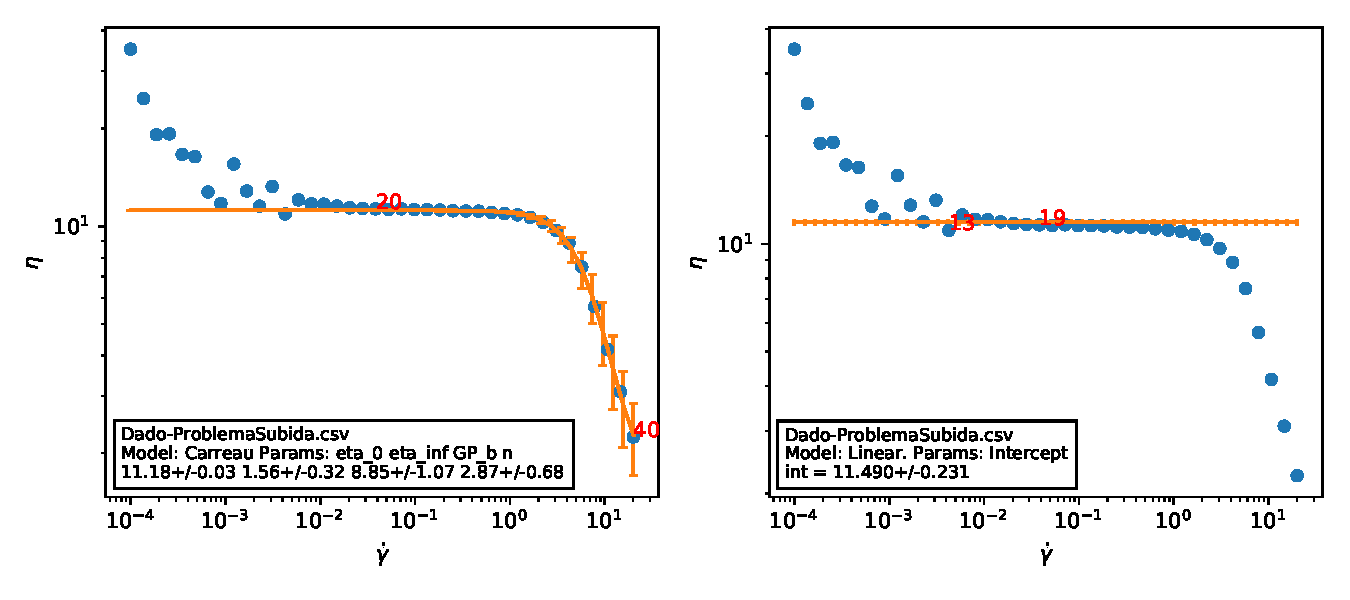
\includegraphics[width=\textwidth]{imagens/reologia/Dado-ProblemaSubida}
			\caption{Exemplo dos ajustes não-linear e linear de um dado real que possui um aumento nos valores de \(\eta\) em baixas \(\dot{\gamma}\)}
			\label{fig:reologia_dado-problemasubida}
		\end{figure}
		
		O tempo de execução e de plotagem para cada experimento está na faixa de um segundo, o que é muito mais rápido do que realizar o ajuste manualmente em uma ferramenta como o Origin ou Excel, então é algo ideal para o tratamento de um grande volume de dados.
		

		\section{Método de ajuste para reologia oscilatória de muco}
		
		As amostras de muco não seguiram modelos de reologia parecidos aos apresentados neste trabalho, como o modelo de Maxwell. Portanto, foi necessário desenvolver uma nova abordagem para analisar as amostras. Plotando-se todos os dados obtidos, observou-se que G' estava sempre acima de G'' e, na escala logarítmica, as duas curvas eram praticamente paralelas e ligeiramente inclinadas positivamente. Em alguns casos, a inclinação aumentava em frequências maiores e, frequentemente, havia uma oscilação de G' e G'' sem significado físico nessa região. A taxa de aumento era consistente com uma exponencial. Visto isso, foi desenvolvido um script que realiza o seguinte:
		
		\begin{enumerate}
			\item Obter a região de frequência confiável de G' e de G'' para o modelo linear e exponencial. Isso é feito realizando-se ajustes gradativos, do primeiro ponto até um ponto \emph{n}, armazenando os ajustes e depois escolhendo o ajuste com maior número de pontos onde \(R^2 > 0{,}9\). Caso não exista ajuste seguindo esse critério, escolhe-se um novo critério com \(R^2 > 0,85\). Caso não exista ajuste que obedeça isso mesmo assim, é escolhido o ajuste com o maior número de pontos. 
			\item Os parâmetros dos ajustes que passaram pelo filtro de \(R^2\) são gravados em um arquivo \texttt{csv}. Além disso, são gravados a média dos valores de G' e G'' da região linear, o desvio dessa média, o valor de \(R^2\), os índices dos pontos utilizados para o ajuste e o valor de G' e G'' em 0,6813Hz. Esses parâmetros foram escolhidos com base em alguns artigos da literatura. % todo: ref?
		\end{enumerate}
		
		Cerca de 500 dados experimentais únicos são tratados e plotados em cerca de 3 minutos, mostrando novamente o ganho enorme de eficiência com métodos computacionais. Após análise estatística, observou-se uma variação significativa em um dos conjuntos de dados. Porém devido à enorme variabilidade das amostras, houve pouca relevância estatística no resto do conjunto de dados. Contudo, os pacientes revelaram uma melhora física após o tratamento estabelecido, mostrando que de fato o tratamento foi eficiente. Mais informações sobre esse projeto podem ser encontrados na tese da aluna. O código fonte da parte de tratamento de dados está nas listagens \ref{lst:extracao_muco1} -- \ref{lst:extracao_muco6}. % todo: colocar uma referência pra tese dela.
		
		\begin{listing}[H]
			\inputminted{python}{./python/extracao_muco1.py}
			\caption{Código fonte para a extração de informações de reologia oscilatória de muco (1/6)} 
			\label{lst:extracao_muco1}
		\end{listing}
		
		\begin{listing}[H]
			\inputminted{python}{./python/extracao_muco2.py}
			\caption{Código fonte para a extração de informações de reologia oscilatória de muco (2/6)} 
			\label{lst:extracao_muco2}
		\end{listing}
		
		\begin{listing}[H]
			\inputminted{python}{./python/extracao_muco3.py}
			\caption{Código fonte para a extração de informações de reologia oscilatória de muco (3/6)} 
			\label{lst:extracao_muco3}
		\end{listing}
		
		\begin{listing}[H]
			\inputminted{python}{./python/extracao_muco4.py}
			\caption{Código fonte para a extração de informações de reologia oscilatória de muco (4/6)} 
			\label{lst:extracao_muco4}
		\end{listing}
		
		\begin{listing}[H]
			\inputminted{python}{./python/extracao_muco5.py}
			\caption{Código fonte para a extração de informações de reologia oscilatória de muco (5/6)}
			\label{lst:extracao_muco5}
		\end{listing}
		
		\begin{listing}[H]
			\inputminted{python}{./python/extracao_muco6.py}
			\caption{Código fonte para a extração de informações de reologia oscilatória de muco (6/6)} 
			\label{lst:extracao_muco6}
		\end{listing}
		
		\chapter{Resultado da colaboração}
		
		OsObservou-se mudanças significativas na reologia oscilatória, mas não nas curvas de fluxo. Observou-se bastante correlação com a variação do pH. Além disso, todos os pacientes reportaram se sentir melhor após o tratamento, a taxa de infecção bacteriana diminuiu, devido ao aumento do pH, e alguns pacientes saíram da fila de transplante. Esse é o primeiro estudo em humanos realizado com bicarbonato, demonstrando a potencialidade da técnica para a melhoria do estado de pacientes com fibrose cística.
		
		Um artigo foi escrito, que será publicado na XYZ % todo: colocar o nome da revista
		
		
%	\chapter{Previsão de temperaturas de fusão de triacilglicerídeos}
%		\section{Breve descrição}
%		\section{Contribuição}